% This is samplepaper.tex, a sample chapter demonstrating the
% LLNCS macro package for Springer Computer Science proceedings;
% Version 2.20 of 2017/10/04
%
\documentclass[runningheads]{llncs}
%
\usepackage{graphicx}
\usepackage{tabularx}
% Use titling to display the title centered on the first page (https://tex.stackexchange.com/questions/290432/vertically-center-title-page-article)
\usepackage{titling}
% Use biber and bibLaTeX
\usepackage[sorting=none, backend=biber]{biblatex}
\addbibresource{bibliography.bib}
% Used for displaying a sample figure. If possible, figure files should
% be included in EPS format.
%
% If you use the hyperref package, please uncomment the following line
% to display URLs in blue roman font according to Springer's eBook style:
\usepackage{hyperref}
\renewcommand\UrlFont{\color{blue}\rmfamily}
\setcounter{tocdepth}{3}
\renewcommand\maketitlehooka{\null\mbox{}\vfill}
\renewcommand\maketitlehookd{\vfill\null}

\begin{document}
%
\title{Introduction to Membership Inference Attacks}
%
%\titlerunning{Abbreviated paper title}
% If the paper title is too long for the running head, you can set
% an abbreviated paper title here
%
\author{Lukas Gehrke \\
\email{lg58weky@studserv.uni-leipzig.de} \\
Leipzig University \\
}
%
\authorrunning{Lukas Gehrke}
% First names are abbreviated in the running head.
% If there are more than two authors, 'et al.' is used.
%
%

\maketitle
% typeset the header of the contribution
%

\tableofcontents
\newpage

\begin{abstract} 
    With more and more companies offering Machine Learning as a Service (MLaaS) a novel threat of data breaches has emerged: Membership Inference Attacks aim at identifying the fact that given data instances were among the training data of a machine learning model available to an adversary. This knowledge might be of fatal consequences, if the membership exposes sensitive information about people, such as a disease or financial dept. This paper gives a general introduction about membership inference attacks. After discussing enabling factors and underlying theory, core studies as well as mitigation strategies are surveyed, followed by a discussion.
    
    \keywords{Membership Inference Attacks  \and Machine Learning Security \and Machine Learning as a Service}
\end{abstract}
%
%
%
\section{Introduction}

\subsection{Machine Learning}

With computers, automation is one of the most simple yet impactful aims that can be achieved.
However, teaching computers to solve complex tasks automatically is hard, as it would require huge amounts of instructions and decision rules for the computer. In order to avoid that, computers are programmed to "learn" the rules on their own using Machine Learning models. A model's learning process is based on experience \cite{mitchell1997machinel}, which again comes from \textbf{data}, called \textit{training data}. If with experience, that is to say appropriate data, a model gets better at its task, it is said to have successfully "learned".

\subsection{Machine Learning as a Service}

Thanks to vast scientific efforts, Machine learning is applicable for many use cases nowadays. These range from simple classification of objects to complicated recognition of signals, such as visual or audio detection. Consequently, numerous possibilities for companies have emerged to improve their products, services or internal processes. However, infrastructure for machine learning is expensive, as huge amounts of data have to be stored and transferred and many calculations have to be conducted. To address these problems, the market of \textbf{Machine Learning as a Service} (MLaaS) has emerged \cite{ribeiro2015mlaas}. The idea behind MLaaS is similar to Software as a Service: A customer has access to remote hardware and software running on this hardware, so that the customer has no need to own them. Examples of companies offering MLaaS are Amazon, Google, IBM or Microsoft. These companies already need the infrastructure and knowledge to process huge amounts of data for their own services. With MLaaS, they gain additional profit by renting hardware that is not fully occupied.

\subsection{Membership Inference}

With ready-to-use machine learning models being used and often being accessible online, a new kind of privacy risk has evolved: The \textit{Membership Inference Attack}. \textit{Membership Inference} asks the simple question, whether a given data record was used to train a machine learning model in question \cite{shokri2017membership}. This leads to critical privacy breaches, if membership in the training dataset allows to imply certain facts. For example, when considering a model that uses cellular structure to recommend ideal medicine dosage for a disease, membership of a person's record in the training data reveals that the person is suffering from this very disease.

This report first explains the theoretical foundation of membership inference attacks. Afterwards, already conducted studies about membership inference attacks are surveyed. Finally, mitigation strategies are discussed, followed by a discussion.

The explanation of theoretical foundations of a membership inference attack are mainly based on the publication by Shokri et al. \cite{shokri2017membership}, who first defined the attack concept. They introduced an architecture based on an attack machine learning model and shadow machine learning models which imitate the behavior of the target model and create training data for the attack model.

\section{Membership Inference Attacks}

The idea behind membership inference attacks is to make use of the fact that machine learning models often exploit different behaviors on previously unseen data in comparison to the data they were trained on\footnote{In the following sections, these two sets of data will be referred to as \textit{testing} and \textit{training data}.} \cite{shokri2017membership}. The main reason for this phenomenon is \textit{Overfitting}. Overfitting describes the tendency of machine learning models or statistical classification models to perform significantly better on their training data in comparison to data they have not been trained on \cite{weigend1994overfitting}. That is to say, the model fails to generalize to data records apart from its training data. Often, this effect is caused by training data with low degree of diversity. The model then does not to learn enough information about the underlying population of the data, as its learning sample is not representative.
Model selection also influences the success of membership inference: Some models \textit{remember} more details about their training data, leading to more leakage of information.

\subsection{Formal Definition}

\subsubsection{Prerequesits}
In this report, \textbf{Membership Inference} is defined as the (theoretical) \textit{question}, whether a given data record was part of the training data of a given, ready-to-use machine learning model. A \textbf{Membership Inference Attack} describes the (theoretical) \textit{act} of performing membership inference against a machine learning model the adversary does not know the training data for and which - if successful - leads to potentially harmful privacy breaches.

\subsubsection{Machine Learning Models}

As introduced by Shokri et al. \cite{shokri2017membership}, the basic membership inference attack setup consists of three machine learning models:
\begin{enumerate}
    \item The \textbf{target model} is the model under attack. The attacker has access to the target model but does not know its exact training dataset.
    \item The \textbf{attack model} performs membership inference by deciding, whether the attack model's output using a given record as input, was part of the training dataset of the attack model.
    \item The \textbf{shadow models} imitate the target model as good as possible. They are used to teach the different reactions of the target model to seen and unseen data to the attack model.
\end{enumerate}

\subsubsection{Attack Definition}

Let $f_{target}()$ be the target model and $f_{attack}()$ be the attack model. $D_{train}^{target}$ is the training dataset of $f_{target}()$, consisting of data records $(\textbf{x}^{i},y^{i})$, with $|D_{train}^{target}| = n$, $i \in (1, \dots , n)$. Here, $\textbf{x}^{i}$ is a vector describing an entity and $y^{i}$ refers to the class of the entity with respect to the task of $f_{target}()$. Assume the number of possible classes for the target model is $c_{target}$. The output of the target model is a vector of values of size $c_{target}$ with each value being in $[0, 1]$ and indicating the probability that the entity in question belongs to the respective class. The vector is denoted by $\textbf{y}_{train}^{i}$.
\par
The attack model $f_{attack}$ uses labeled data entries and the respective outputs generated by the target model for these entries as input $x_{attack}$. Its purpose is to recognize whether a data entry was part of the training dataset based on these inputs. This task leads to a binary output scheme: "\textit{in}" for data records of the training dataset and "\textit{out}" for non-members.
The attack procedure is as follows: For a labeled data record $(\textbf{x}, y)$ the output of $f_{target}()$ is generated: $f_{target}(\textbf{x}) = \textbf{y}$. Afterwards, the tuple $(y, \textbf{y})$ is queried to the attack model. Ideally, the attack model then recognizes patterns in distribution of $\textbf{y}$ around the actual $y$ \cite{shokri2017membership}. The attack model then calculates the pobability $P(((\textbf{x}, y) \in D_{train}^{target})$ that the record $(\textbf{x}, y)$ was part of the training dataset of the target function or belongs to the "\textit{in}" class. Figure \ref{fig:attack} gives an overview over the attack procedure. Note that it would also be possible to use only $\textbf{y}$ or to use $((\textbf{x}), \textbf{y})$ as input for the target model. In the latter case the model could identify patterns in the relationship between $\textbf{x}$ and $\textbf{y}$.

\begin{figure}[ht]
    \centering
    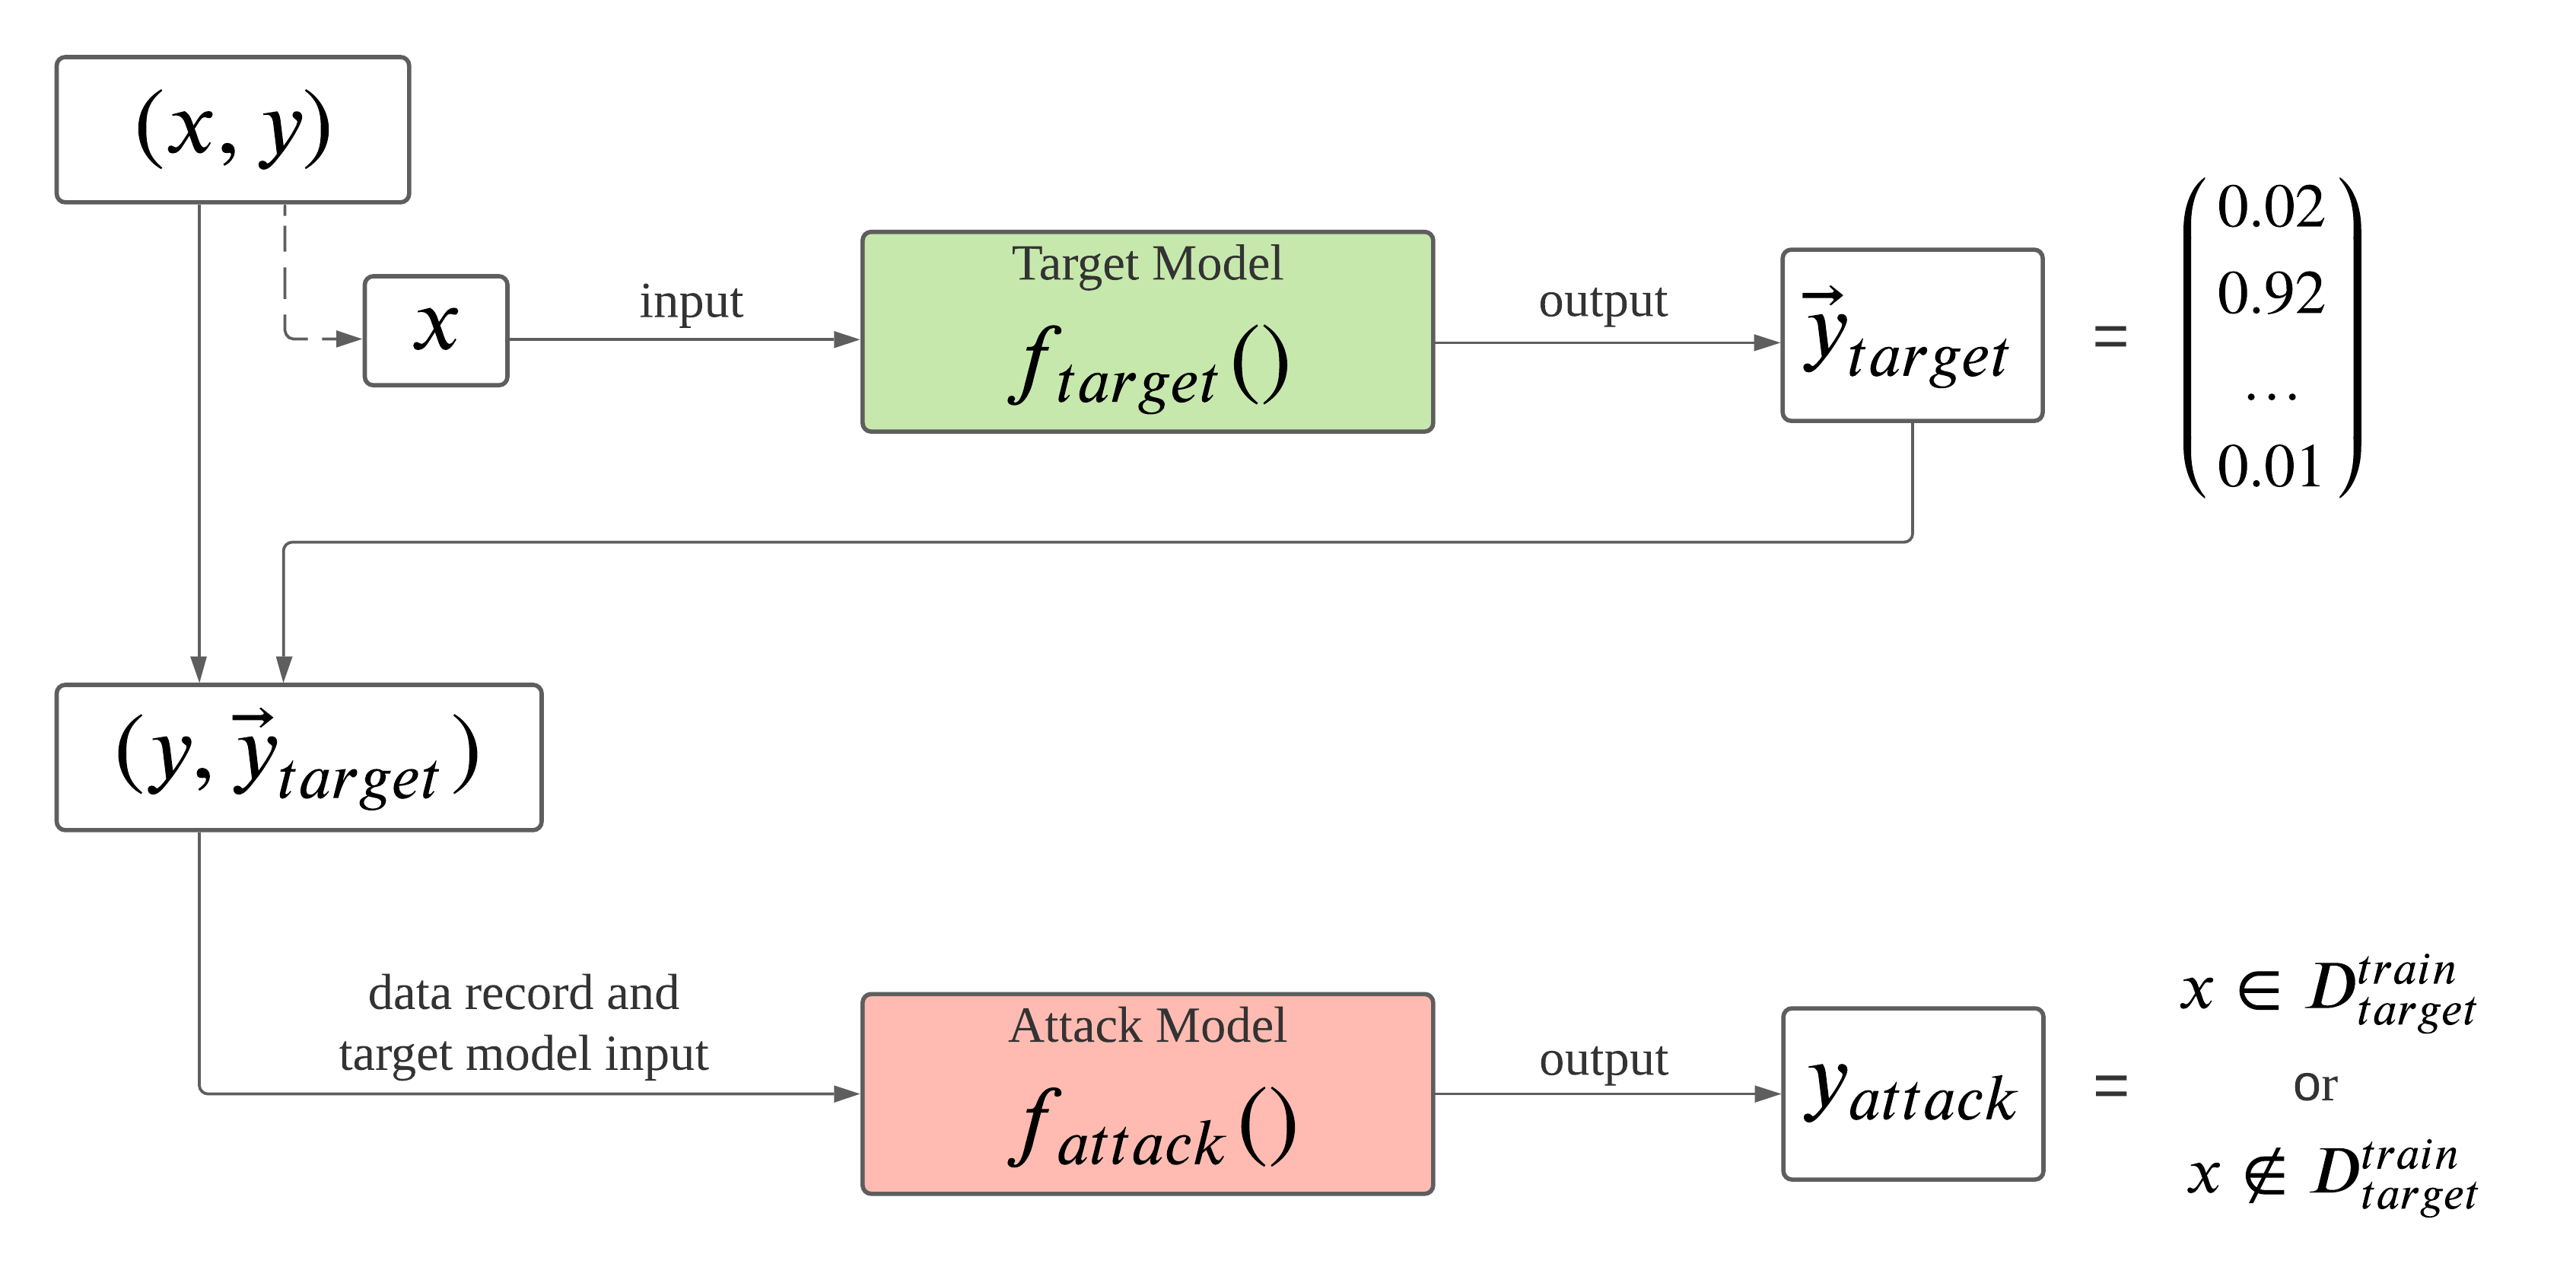
\includegraphics[scale=0.1]{figures/mia-black-box-attack.png}
    \caption{The black-box Membership Inference Attack scenario. A data record $(\textbf{x}, y)$ is first queried to the target model. Afterwards, the output and of the target model and the true class of the data record are used as input for the attack model. The attack model decides, whether the data record was in the training dataset of the target model or not.}
    \label{fig:attack}
\end{figure}

\subsubsection{Attack Model Training}

One fundamental part of the aforementioned process remains open: The training of an attack model. Therefore, Shokri et al. \cite{shokri2017membership} propose a technique called "\textit{shadow training}". Multiple shadow models $f_{shadow_{i}}()$ are generated with the main aim being to make their behavior as similar to the target model's behavior as possible. The training datasets $D_{train}^{shadow_{i}}$ are all known and may partially overlap. Training data for the shadow models may originate from existing sources. Otherwise data records have to be generated as "\textit{synthetic}" training data. The idea of using synthetic training data is based on empirical evidence following the idea that similar machine learning models provided by the same service and trained on similar data behave similarly \cite{shokri2017membership}. Moreover, Shokri et al. claim that a higher amount of shadow models provides more training experience for the attack model and thus enhances the attack accuracy.
To generate training data for the shadow models, Shokri et al. \cite{shokri2017membership} propose different methods:

\begin{itemize}
    \item \textbf{Model-based Synthesis} uses the target model for the generation of synthetic training data. It is based on the idea that if the target model classifies a randomly generated data record with high confidence, that is to say with a value close to $1$ for the predicted class and with values close to zero for all other classes, the data record is similar to a real entry from the target models training data.
    \item \textbf{Statistics-based Synthesis} bases generation of synthetic data on statistical knowledge about the underlying population of the training dataset of the target model.
    \item \textbf{Noisy real data}: If real data records of the training dataset of the target model are accessible, these can be used to generate new records by changing a selected number of random properties of the records at hand.
\end{itemize}

The Model-based synthesis as introduced by Shokri et al. \cite{shokri2017membership} uses a two-phase process: First, records that are classified by the target model with high confidence are searched. This procedure is iterative and involves randomly initializing data records. Afterwards, features are changed until the prediction confidence by the target model for a fixed class surpasses the confidence for all other classes and a threshold. Additionally, already accepted synthetic records are used as a base for new ones. In each iteration, a new record is created by randomly changing features of the last accepted record. The second phase consists of sampling new records for the synthetic datasets if the acceptance criteria from phase one are met.
\par
To train the attack model, each shadow model $f_{shadow_i}()$ has to classify all records of its respective training dataset $D_{shadow_i}^{train}$ and test dataset $D_{shadow_i}^{test}$. Given a record $(\textbf{x}, y)$ from a training set, the output $f_{shadow_i}(\textbf{x}) = \textbf{y}$ will be extended with the label "\textit{in}". Thus, the tuple $(y, \textit{y}, in)$ will be added to the attack model training dataset $D_{attack}^{train}$. Note that $y$, the true label, is added to enable the attack model to learn the distribution of $\textbf{y}$ around $y$ as mentioned earlier. For all entries of $D_{shadow_i}^{test}$, tuples of the form $(y, \textit{y}, out)$ are added to $D_{attack}^{train}$. Afterwards, $D_{attack}^{train}$ is split into $c_{target}$ partitions, one for each value of $y$, the true class label. Then, according to Shokri et al. \cite{shokri2017membership}, for   every class $y_i$ a separate attack model $f_{attack_i}$ should be trained. Figure \ref{fig:attack} illustrates the attack model training process. Ultimately, the resulting task is a binary classification task. This is a standard task in machine learning, allowing the attack model to be build with any machine learning framework. Within this binary classification task, the attack model learns how to keep apart records that belong to the "\textit{in}" or "\textit{out}" group and where \textit{both classified with high confidence by the target model}, as Shokri et al. \cite{shokri2017membership} highlight. A task much subtler than only distinguishing between records classified with high or low confidence, which is not what the attack model learns \cite{shokri2017membership}.

\begin{figure}[ht]
    \centering
    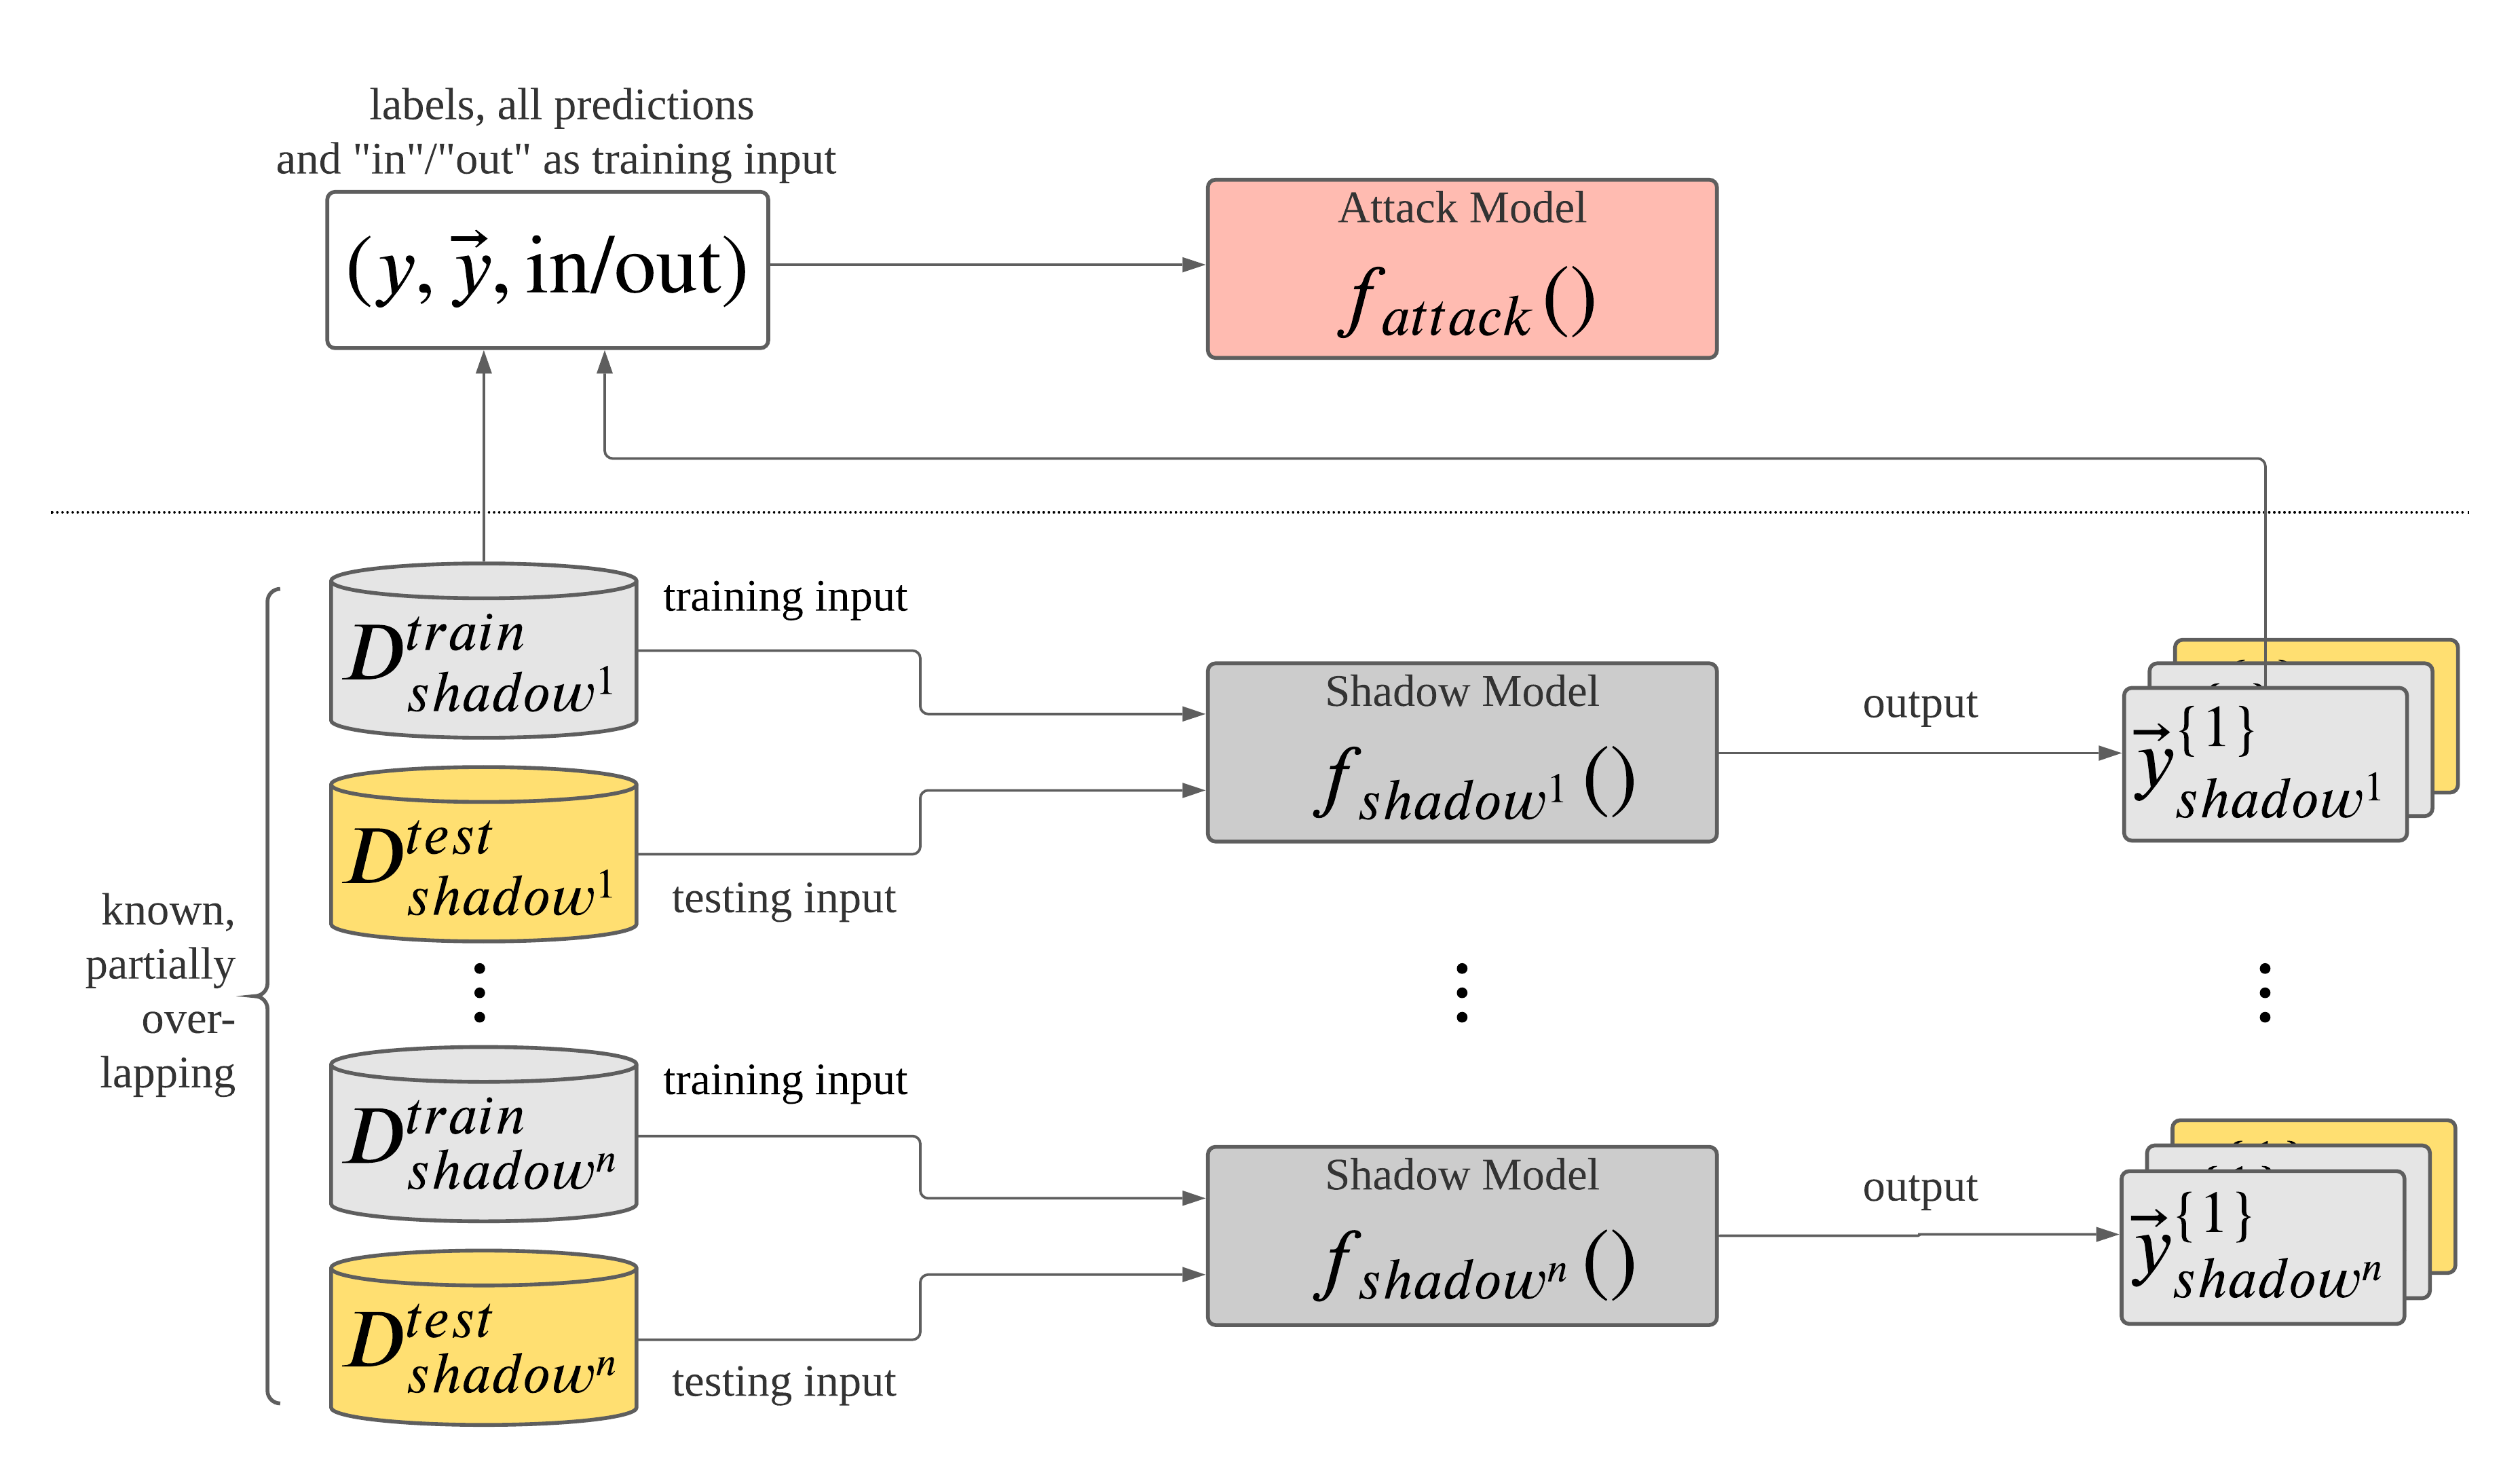
\includegraphics[scale=0.093]{figures/mia-attack-model-training.png}
    \caption{The attack model training process involves $n$ shadow model with partially overlapping training and testing datasets.For every shadow models, all prediction results are obtained and additionally, each result is flagged with "\textit{in}" if the respective record was in the training dataset of the shadow model and "\textit{out}" otherwise. Resulting tuples are extended with a records true class $y$ and then used as training data for the attack model.}
    \label{fig:attack-training}
\end{figure}

\subsection{Scientific Studies}

In this chapter, studies about membership inference attacks are presented. The chapter begins with an overview of most notable scientific publications. Afterwards, key studies are reviewed in detail. As many publications include a chapter about mitigation strategies, these are also mentioned in the overview. Mitigation strategies are discussed later on.

\subsubsection{Overview of Studies}

Several studies about membership inference attacks have been conducted.
Shokri et al. \cite{shokri2017membership} use six different datasets and 4 different target models to explore the possible threats of membership inference attacks. They find out that machine learning models indeed leak information about their training data and show the success of their shadow model training technique. They also discuss multiple mitigation techniques such as regularization or restriction of the prediction vector.
Truex et al. \cite{truex2018towards} directly tie on this work by developing a framework for membership inference attacks. They survey attacks against different types of machine learning models and explore the success factors of membership inference attacks. A study of mitigation strategies such as model hardening and differential privacy is also conducted, revealing need for more studies on this matter. 
Hayes et al. \cite{hayes2017logan} focus on attacks against generative machine learning models, a version of neural networks that is very popular in many applications nowadays. Generative adversarial networks use a combination of a discriminative and a generative model and are mostly used to generate images or videos \cite{goodfellow2014generative}. Hayes et al. show that membership inference attacks work better against discriminative models than against generative models. Moreover, they experiment with regularization techniques as mitigation strategies and report mixed success as well as need for more research on that topic.
Salem et al. \cite{salem2018ml} study applicability of membership inference attacks by gradually reducing the assumptions on the attack model. They experiment with a lower amount of shadow models and attack training data generation through so-called data transferring attacks. They also explore means of reduction of overfitting to oppose membership inference attacks.
Jia et al. \cite{jia2019memguard} develop a defense framework against membership inference attacks. The framework enables adding noise to output vectors of potential target models in order to confuse attack models.

\subsubsection{Original Studies}

Shokri et al. \cite{shokri2017membership} use six datasets to explore the possibilities of membership inference attacks against different target models. Table \ref{tab:datasets-shokri} gives an overview of the datasets. As target models, they use three MLaaS models and one model that is implemented locally. The models are listed in table \ref{tab:target-models-shokri}.

\begin{table}[ht]
    \centering
    \begin{tabularx}{\textwidth}{|l|l|X|c|}
        \hline
        \textbf{Dataset} & \textbf{Task} & \textbf{Features} & \textbf{Entities} \\
        \hline
        \textbf{\href{https://archive.ics.uci.edu/ml/datasets/adult}{UCI Adult}{}} & Binary classification & 14 features (binary and numerical) &  48,842 \\
        \textbf{\href{https://www.kaggle.com/c/acquire-valued-shoppers-challenge/data}{Purchases}{}} & 2 to 100 class classification & 600 binary features & 197,324 \\
        \textbf{\href{https://www.cs.toronto.edu/~kriz/cifar.html}{CIFAR}{}} & 10 to 100 class classification & 32 x 32 color images & 60,000 \\
        \textbf{\href{http://yann.lecun.com/exdb/mnist/}{MNIST}{}} & 10 class classification & 32 x 32 images of handwritten digits & 70,000 \\
        \textbf{\href{https://sites.google.com/site/yangdingqi/home/foursquare-dataset}{Locations}{}} & 128 class classification & 446 binary features & 11,592 \\
        \textbf{\href{https://www.dshs.texas.gov/THCIC/Hospitals/Download.shtm}{Hospital Stays}{}} & 100 class classification & 6,170 binary features & 67,330 \\
        \hline
    \end{tabularx}
    \caption{Overview of the datasets initially used to study membership inference attacks \cite{shokri2017membership}}
    \label{tab:datasets-shokri}
\end{table}


\begin{table}[ht]
    \centering
    \begin{tabularx}{\textwidth}{|l|X|}
        \hline
        \textbf{Model} & \textbf{Parameters} \\
        \hline
        \textbf{\href{https://cloud.google.com/ai-platform}{Google Prediction API}} & No configuration parameters available \\
        \textbf{\href{https://aws.amazon.com/machine-learning/}{Amazon ML} version I} & maximum number of passes over the training data, L2 regularization amount: $(10, 1e - 6)$ \\
        \textbf{\href{https://aws.amazon.com/machine-learning/}{Amazon ML} version II} & maximum number of passes over the training data, L2 regularization amount: $(100, 1e - 4)$ \\
        \textbf{Neural networks} & \href{https://github.com/torch/nn}{Torch7}, Convolutional neural network with two convolutions and max pooling layers, fully connected layer of size 128, SoftMax layer \\
        \hline
    \end{tabularx}
    \caption{Overview of the machine learning models used in the initial publication about membership inference attacks \cite{shokri2017membership}}
    \label{tab:target-models-shokri}
\end{table}

Shokri et al. \cite{shokri2017membership} use precision and recall as well as accuracy as measures of attack success. Precision is defined as the fraction of records the attack model identifies as members of the training dataset that indeed are members. Recall is defined as the fraction of the training dataset that is correctly identified by the attack.
\par
First, the accuracy of the attack is measured. The measurement is based on training and testing datasets of the same size, thus the baseline accuracy is $0,5$. On the neural-network, the authors report a high degree of overfitting when measuring test dataset accuracy with the CIFAR dataset. The train-test accuracy gap on the CIFAR dataset is $0.5$ when using Amazon ML version II. Regarding the attack precision, on the CIFAR dataset with ten classes (CIFAR-10), the median precision is $0.72$ for a training set size of $10,000$. For the CIFAR-100 dataset, the precision is almost $1$, while recall is almost $1$ for both scenarios. Against the Google model, the precision is even higher in the same setup.
On the Hospital Stays and Locations dataset, Shokri et al. \cite{shokri2017membership} evaluate an attack against the Google model, reaching precision of more than $0.7$ for half of the classes and a precision between $0.6$ and $0.8$ respectively.
\par
Furthermore, the \textit{effect of the different shadow model training techniques} was studied. For the noisy training data, precision is reported as dropping with increasing noise. However, the authors note that with noisy data the attack precision is still above baseline. Therefore they deduce that membership inference attacks even work with vague assumptions about the training data.
To evaluate the approach of model-based synthesis on the Purchase dataset, $30,000$ fully synthetic records and $187,300$ marginal-based synthetic records are generated. The marginal-based approach uses marginal distributions of individual features to generate synthetic data. For the fully synthetic records, on average $156$ queries to the target model are needed in order to generate a single entry. Against the Google model with black-box access, the attack precision and recall are $0.935$ and $0.994$ for real-data, $0.896$ and $0.526$ for model-based synthetic data as well as $0.795$ and $0.991$ for the marginal-based synthetic data. The authors mention that the attack model performs very poorly on some classes when being trained on the model-based synthetic data. This effect might be due to the under-representation of some classes in the target-models training dataset, leading to bad synthetic records. Overall, Shokri et al. \cite{shokri2017membership} report that membership inference attacks perform very well even without any knowledge about the data in the training dataset of a black-box-access target model. A prerequisite is the ability of an adversary to access the target model and obtain predictions with high confidence from it.
\par
Additional studies by Shokri et al. focus on the "\textit{effect of the number of classes and training data per class}" and the consequences of \textit{overfitting} for attack success. The authors claim that the more classes, the better a membership inference attack works. A study using the Purchases dataset and the Google model supports this claim. While with $20$ classes average precision is around $0.6$, with 50 classes average precision rises to almost $0.9$. The authors try to explain this effect by analyzing the behavior of the target model. With more classes, the model has to use more separating information from the records to be able to distinguish inputs from the different classes accurately. Thus, the model leaks more information.
\par
Finally, the effect of overfitting is considered with a calculation of the train-test accuracy gap. Overfitting is directly related to a high train-test accuracy gap, because a high gap indicates that the model in question fails to generalize from its training data to the test data and is thus overfitted. Shokri et al. identify a positive correlation between the size of the accuracy gap of a model and the accuracy of the membership inference attack against the same model. However, they also find counter-examples, where a model with a smaller accuracy gap is more vulnerable to membership inference attacks.
The authors conclude that overfitting and diversity of training data straightly enable success of membership inference. They thereby identify privacy leakage as another negative effect that overfitting causes for machine learning models next to performance loss.

\subsubsection{Further Studies}

Following the initial paper about membership inference attacks, Truex et al. \cite{truex2018towards} conduct experiments with the same datasets, Adults, MNIST, CIFAR and Purchases. Additionally, they carefully define the attack setup and process. They highlight that the training dataset of the target model heavily influences the success of an attack: The higher the number of classes and the higher the in-class standard deviation, the higher the accuracy of a membership inference attack. They explain the effect of the number of classes with the underlying space ${\rm I\!R}$ of the dataset, that they assume to be more and more divided for higher numbers of classes. This would result in smaller areas for single classes and the areas would more closely frame the single data records from the associated class. Consequently, the borders between class areas become much and much smaller with all records being closer to the borders. This results in higher influence of single records on the decision borders. Thus, Truex et al. argue, an adversary would identify a data record with higher probability as the model under attack would more likely be "\textit{impact}(ed)" by the instances for its decisions.
Regarding the in-class standard deviation, Truex et al. claim that higher standard deviation inside a class favors membership inference attacks. They argue that if records within the same group have huge differences, then the consideration of every single instance will influence the decision structure of the target model.
The authors underpin their claims with a comparison of the aforementioned datasets using the respective in-class standard deviation, number of classes and attack accuracy. In general they claim that the higher the complexity of the classification problem, the higher the accuracy of an attack and that success of membership inference attacks is driven by the underlying data of the target model. They add that some factors may be dominant over others, as they find Purchases-100 to result in higher attack accuracy than Purchases-50 while the in-class standard deviation is nearly equal.
Additionally, they study the selection of model type for all three models involved in an attack: The target model, the attack model and the model for attack model data generation ("shadow model"). The experiments involved measurement of attack accuracy and standard deviation in attack accuracy with changing models. They reveal that attack success depends on the target model while the other models are interchangeable. Therefore, the authors described membership inference attacks as "\textit{transferable}" \cite{truex2018towards}. As a consequence, an adversary might create a successful attack model without the knowledge about the best model type for membership inference.
Moreover, Truex et al. study the influence of the knowledge of an attacker about the target data, similarly to the experiments by Shokri et al. with noisy data. The receive similar findings: Even with $10\%$ data loss, features replaced by random values ("noise"), attack accuracy remains high. When inspecting the shadow model training data, they find a similar noise resilience. They furthermore suggest that shadow model training datasets should be sufficiently large, as they find some significant increases in performance when carrying out experiments on the Purchases-20 and 50 datasets with varying shadow model training dataset sizes.
To sum up, Truex et al. report new insights about membership inference attacks such as that the attacks are mainly influenced or enabled by the target model and the underlying data and that attack and attack data generation models are interchangeable.
\par
Hayes et al. \cite{hayes2017logan} focus on membership inference attacks against generative machine learning models. They again use CIFAR-10 as well as Labeled Faces in the Wild (LFW), a dataset consisting of images with faces and Diabetic Retinography (DR), consisting of images of retinas. The authors perform white-box and black-box attacks against three different generative adversarial networks (GAN) with one fixed GAN as attack model. They also used a black-box setting with limited auxiliary knowledge: Here, an adversary has knowledge of about $20-30\%$ of the training or testing set of the target model. The black-box attack without and with auxiliary knowledge on the LFW dataset yields an accuracy of $0.4$ and $0.63$ respectively. With the CIFAR-10 dataset, accuracies $0.37$ and $0.58$ respectively are reached, while $0.22$ and $0.81$ are the results on DR. Note that random guessing yielded $0.1$ accuracy on LFW and CIFAR-10 and $0.2$ on DR. Additionally, Hayes et al. \cite{hayes2017logan} underpin the finding of Truex et al. \cite{truex2018towards} that different attack models yield similar attack performance.
Moreover, the authors claim that attack accuracy is directly correlated to with the quality of generated training data for the attack model. They report that the target model, if used for data generation, generates better data than an attack data generation model and that in general better training data is created after more training epochs of the models.
All in all, Hayes et al. show that membership inference attacks against GANs are possible and discover techniques to improve attack performance.
\par
Salem et al. \cite{salem2018ml} simplify membership inference attacks by removing multiple requirements towards the adversary. First, they perform membership inference using only one shadow model in contrast to Shokri et al. \cite{shokri2017membership} using the same datasets.
Notably, their attack with only one shadow model yields almost equal performance regarding precision and recall on all datasets.
They also study the need of knowledge about the structure of the target model. By changing the parameters of the target neural network model and performing an attack using the Purchase-100 dataset, they receive similar results despite changed parameters. 
Therefore, the authors claim that knowledge about the hyperparameters of a target model is not required to perform the attack. 
To test the influence of knowledge about the classification algorithm of the target model, Salem et al. created a shadow model that combines different algorithms. Thereby, the behaviors of all algorithm can be taught to an attack model with one shadow model. They combine logistic regression, multilayer perceptron and random forests and evaluate the combined model on the Purchase-100 dataset against each of these algorithms alone as target model. Moreover, they use a single shadow model against each target model, always with the same algorithm as the target, for comparison. The results indicate that the combined model performs similarly to the respective single models, revealing only a little skew for random forests as target algorithm.
A second study by Salem et al. introduces a novel technique for synthetic attack data generation. Here, the shadow model generates training data for the attack model independently from the distribution of the target models training data. The underlying idea is to only teach the attack model general knowledge about membership and non-membership in a training dataset of a target machine learning model. In their experiment, the authors randomly pick on of the datasets for attack data generation and one as target training dataset and overall receive precision of more than $0.7$ and similar rec  all, although there are some outliers. The authors claim that this procedure also simplifies generation of attack training data, as huge amounts of queries against the target model become unnecessary.
The third approach by Salem et al. focusses on minimizing all requirements to the attack model by completely withdrawing shadow models and using unsupervised binary classification \cite{salem2018ml}. The authors claim that membership inference with solid accuracy is even possible in this setting.
Overall, Salem et al. present some effective simplifications for membership inference attacks such as the reduction of the amount of shadow models or the usage of training data for attack data generation, that is completely unrelated to the target dataset.

\subsection{Mitigation Strategies}

In order to prevent membership inference attacks, several studies share their insights about the best mitigation strategies.
Shokri et al. \cite{shokri2017membership} discuss four techniques: They (1) leave out classes with low probability from the prediction vector, (2) round the values in the prediction vector, (2) increase the output vector's entropy and (3) apply regularization. Regularization aims at reducing model complexity, so that the fit of the model to its training data, especially outliers, is not to tight \cite{ng2004feature}. The authors find their membership inference attacks to withstand most of their mitigation attempts. For example, leaving out classes of the prediction vector, even reducing the number of output classes to 1, the class with the highest probability does not decrease attack accuracy significantly. Shokri et al. report regularization as the only useful technique but at the same time warn to not over-use it to prevent the potential target model from losing its prediction performance.
Truex et al. \cite{truex2018towards} present "\textit{model hardening}" and "\textit{API hardening}" to prevent membership inference attacks. In case of model hardening, they suggest (1) choosing a machine learning model or algorithm that is resilient against membership inference, (2) controlling their model while training in order to prevent overfitting, e.g. by using certain model parameters, (3) applying regularization and (4) apply anonymization techniques. With API hardening, Truex et al. describe techniques that affect the working model in use. Here, they recommend techniques similar to Shokri et al. \cite{shokri2017membership}. Moreover, they recommend usage of differential privacy mechanisms. 
Hayes et al. \cite{hayes2017logan} study usage of "\textit{Weight Normalization}" and "\textit{Dropout}". They report Dropout to be way more effective than Weight Normalization but also claim that Dropout significantly prolongs the training phase. Similarly to Truex et al. they also study differential privacy mechanisms.
Salem et al. \cite{salem2018ml} introduce "\textit{model stacking}" as mitigation strategy in addition to Dropout, which is only applicable to neural networks. This technique uses ensemble learning to split training of the components of a potential target model with different parts of the training dataset. Thereby, Salem et al. want to reduce to degree of overfitting of the model. Their experiments conducted with model stacking revealed reductions of attack performance on different datasets of up to $30\%$ and more.
To sum up, different privacy preserving techniques are researched, ranging from simple reduction of model output complexity over implementation of new model training procedures up to privacy systems such as differential privacy.

\section{Conclusion}
\subsection{Summary}

Machine Learning offers many possibilities to create new services or simplify existing ones but also has high requirements regarding hardware, software and know-how. With Machine Learning as a Service, the possibilities of machine learning have become accessible for a broad range of institutions. However, large amounts of data underlie these systems and are the basis for successful learning. Often, these data are privacy-sensitive. MLaaS and the potential privacy-sensitivity of underlying data have caused a new threat for privacy: Membership Inference Attacks - the identification of the fact that a given data record was used to train a machine learning model at hand.
\par
This report gives a general introduction about the developments that made membership inference attacks possible, the theoretical process of performing an attack with an attack model and shadow models as well as an overview of key studies about membership inference attacks and related defense strategies.

\subsection{Discussion}

Membership inference attacks offer an interesting field of studies. In some studies, single questions remain open.
Shokri et al. \cite{shokri2017membership} claim that the more shadow models are used for attack data generation, the more accurate the attack model will be. However, they provide no empirical evidence for their claim. Moreover, Salem et al. \cite{salem2018ml} show that a single shadow model offers similar performance in comparison to multiple shadow models. Therefore, the aforementioned un-tested claim in the study by Shokri et al. is simply wrong. The mistake could have been avoided by doing an additional experiment on the number of shadow models.
\par
The discussion of the effect of the number of classes as explained by Truex et al. \cite{truex2018towards} seems to link to the  "curse of dimensionality" defined by Bellman \cite{Bellman:DynamicProgramming}. The curse of dimensionality states that with higher amount of dimensions, a latent space gets larger, increasingly empty and the instances in it gather close together. Following their argumentation, higher numbers of dimensionality of the training dataset under attack should cause higher vulnerability for membership inference attacks, as the instances would get closer together and influence the decision processes of the target model \cite{truex2018towards}.
Truex et al. state that in class standard deviation directly affects membership inference attack success but do not give real empirical evidence for that claim in their publication. In the corresponding table, they even have an example that opposes their hypothesis with CIFAR-10 having lower in-class standard deviation than Purchases-10 but higher attack accuracy. Both examples have 10 classes.
In general, Truex et al. \cite{truex2018towards} seem to replicate or at most refine lot of the work of Shokri et al. \cite{shokri2017membership} such as a giving formal definition of membership inference attacks and their order of events with shadow models which they call "\textit{(...) the first generalized framework for the development of a membership inference attack model}". This is a critical claim, as Shokri et al. \cite{shokri2017membership} introduced a very similar architecture before, though never called it "\textit{framework}". Additionally, Truex et al. \cite{truex2018towards} do not reference Shokri et al. \cite{shokri2017membership} for first finding out that the number of classes is positively correlated with the accuracy of a membership inference attack. Instead, they avoid to directly describe the phenomenon in their publication (chapter 4.2) although it is observable in the table in chapter 4.2.

\subsection{Outlook}

With new machine learning models and refinements of already available models being published all the time, membership inference attacks remain an important topic. Every new model is a potential target model and a potential attack model. Therefore, studies about frameworks for quick checks of vulnerability of new models would be an interesting topic for further research.
In general, the study of mitigation techniques remains important, as the aforementioned studies show, that many mitigation ideas fail to prevent membership inference attacks.
Additionally, topics like the influence of the dimensionality of the data under attack on the attack performance could be addressed in future work.


%
% ---- Bibliography ----
%
% BibTeX users should specify bibliography style 'splncs04'.
% References will then be sorted and formatted in the correct style.
%
% \bibliographystyle{splncs04}
% \bibliography{mybibliography}
%

\printbibliography

\end{document}
